% !TeX spellcheck = en_GB
\vspace{-1cm}
\noindent\rule{\textwidth}{1pt}
%\vspace{-1.5cm}
\begin{abstract} 
\vspace{-0.3cm}
\begin{center}
	{\large\bfseries\sffamily\MakeUppercase{Abstract}}
\end{center}
\noindent
The Black Kite is an abundant bird of prey in Spain. The main goal is to access which site covariates are important for the occurrence of the Black Kite in Spain. Furthermore, an actual distribution map of the Black Kite in Spain is presented and compared to the distribution under the assumption of an increase of annual mean temperature and a decrease of total precipitation in 80 years. The selection of site covariates is based on ecological knowledge of the focal species and an exploratory analysis with a Random Forests model. The eBird data set is filtered for repeated surveys and used as the data source for fitting the static occupancy model. 
\end{abstract}
\vspace{-0.5cm}
\noindent\rule{\textwidth}{1pt}

%\blindtext[3]
\begin{multicols}{2}
	
\section{Introduction}
Climate change affects all levels of biodiversity \parencite{Bellard2012, Garcia2014}. A main task in ecological research is to build accurate models to predict the biological response to climate change \parencite{Urban2016,Araujo2006}. 

One of the affected groups by the climate change are birds of prey. Birds of prey play a crucial role in ecosystems. Very often they are top predators. They can be regarded as flagship species, because they are very vulnerable to human activity, because of their role as top predator in food chains and because of the attractiveness of their behavior to humans. Furthermore, they provide regulating, supporting and cultural ecosystem services \parencite{Donazar2016}.

A raptor species with a very wide distribution is the Black Kite, \textit{Milvus migrans} (Boddaert, 1783). The distribution of this species ranges from Western Europe to East Asia and Australia \parencite{BirdLife2021}. The species is mainly migratory and the European population stays in the winter in sub-Saharan Africa. The individuals leave the breeding area between July and October and come back back between February and May \parencite{Panuccio2014, BirdLife2021}. In this case study the focus lies on the Black Kite population in Spain. 

Citizen science data are often used in species distribution modelling, because of the high data availability. However there are some challenges in using these data sets, for example the spatio-temporal bias of the of the observations. For instance people tend to watch for birds more in the breeding season and around their own home \parencite{Robinson2018, Reich2018}. Two techniques are available to overcome this difficulties. First, it is possible to filter out low quality observations. Second, it is possible to apply statistical techniques to address sampling bias and observational heterogeneity \parencite{Steen2019}. In this study the second option is used. Observational heterogeneity and imperfect detection is tackled with an extension of species distribution model, the so-called occupancy model \parencite{MacKenzie2002}.

The model is used to learn more about the ecology of the focal species. This knowledge can be used in conservation planning.  

The main questions are (1) which site covariates are most important for the occurrence of the Black Kite and (2) what happens to the Black Kite population in Spain under future climate conditions.


\section{Methods}
Data of the species occurrences are from eBird data \parencite{Sullivan2009, ebirdData}. The dataset is filtered for repeated surveys, that were done three to ten times in the same area between April and June of 2019. Only standing or travelling surveys with a total distance up to 5 km with one to five observers were used. To get an overview a map with all observations was produced using \textcite{QGIS_software}.

Data preparation, selection of covariates, model selection, model evalutation and prediction were done with \textcite{R_lang}. Exploratory analysis of the covariates were done in \textcite{python}. An ODMAP-Protocol \parencite{Zurell2020} describing typical steps in species distribution modelling can be found in the electronic appendix.


\subsubsection*{Spatial resolution of the model}
The home range size differs between younger not breeding individuals, that are one to seven years old, so-called floaters, \parencite{Blas2009} and the breeding individuals. Floaters had in south Spain an home range size over 300 km$^2$, breeding females 43 km$^2$ and breeding males 80 km$^2$ \parencite{Tanferna2013}. However, these home range values were observed with radio-tracking of individuals and later on the calculation of the minimum convex polygon. The main activity is probably more restricted to centre of the area.

A resolution of 2.5 minutes (roughly 21.5 km$^2$) was chosen. It is possible to argue that the size is too small for the large home range sizes of the Black Kite. However through spatial subsampling the data loss is higher and the connection between the observations and the site variables becomes less strong.

\subsection*{Selection of detection covariates}
Detection covariates that are present in the eBird data are used. These are the day of the year, time when observation started, duration of observation, walking distance and protocol type (standing or travelling). The two most important covariates from the Random Forests model (see section on exploratory analysis of covariates) were used in the final model. 

\subsection*{Selection of site covariates}

First a preliminary selection of site covariates was compiled. These set include all bioclimatic variables \parencite{Fick2017}, land cover fractions, as the tree cover, the grass cover and the bare soil cover \parencite{land_cover_data}, and the distance between the centre of the raster cells to the closest landfill and the closest river or lake. 

In the next step ecological hypotheses were formulated based on existing ecological knowledge from the literature. Some of the covariates were selected based on these hypotheses. As an additionally step, all preliminary covariates were used to fit a Random Forests model and to get the importance of all the covariates for predicting the detection probability of the Black Kite. The most important covariates from these analysis were added to the list of covariates. 

The covariates from the ecological hypotheses and from the Random Forests model were tested for collinearity with the Variance Inflation Factor \parencite[as implemented in][]{Heiberger2020}. Highly collinear covariates were removed. Maps of the final site covariates can be found in the appendix (see Figure \ref{fig:site_cov_maps}). The complete selection process is shown in Figure \ref{fig:selection_covariates} and further explained in the next sections.  


\begin{minipage}{\linewidth}
	\vspace{1cm}
	\centering
	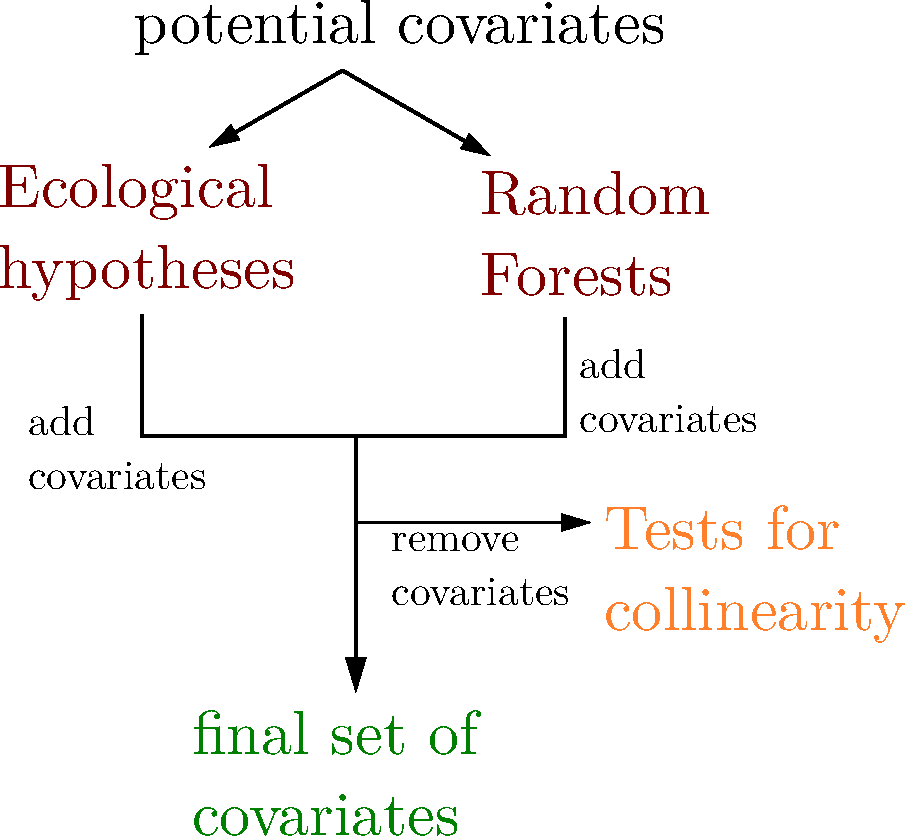
\includegraphics[width=0.9\linewidth]{img/selection_of_cov}
	\captionof{figure}{Procedure of selecting site covariates for the occupancy model}
	\label{fig:selection_covariates}
\end{minipage}

\subsubsection*{Data preparation of site covariates}
For all raster operations \textcite{raster} was used. Bioclimatic variables were download from \textcite{Fick2017} in the target resolution. Tree cover, herbaceous vegetation cover and bare soil cover were downloaded \parencite{Buchhorn2020, land_cover_data}. The raster images were merged to one file and then cropped to mainland of Spain. The resolution was resampled to the target resolution using a bilinear interpolation.

Land cover data was retrieved in vector format \parencite{clc2018} and cropped to the mainland of Spain. The distance between each centre of the raster cell to all polygons of landfills and rivers or lakes was calculated with \textcite{rgeos}. Afterwards, the minimum distance was saved.  


\subsubsection*{Ecological justification of site covariates}
The selection of covariates is based on existing ecological knowledge about the focal species. A list of all site covariates and a corresponding simplified hypothesis can be found in Table \ref{table:covariates}.

The Black Kite uses a variety of feeding sources, for example birds, fish, crayfish, insects, carrion, vegetable matter and smaller mammals \parencite{Sergio1999,Vinuela1992, BirdLife2021}. Part of the prey is found in wetlands and marshes and it was proposed that the Black Kite has a habitat binding to wetlands and marshes \parencite{Veiga1990, Tanferna2013}. Accordingly, the minimal distance to lakes and river was calculated and used as a site covariate. The distance to the closed lake or river was used, because it is more important that lakes or rivers are nearby than that the Black Kite was actually observed in cell with a lake or a river. 

It has been shown that Black Kites visit landfills for feeding \parencite{DeGiacomo2008, Blanco1994}. Therefore the distance to the closest landfill were analysed. The landfill cover was not used, because in most of the raster cells landfills are not present and therefore the model fitting will not be optimal.

Black Kites breed in branches of trees. However, closed woodlands are avoided \parencite{Tanferna2013}. Therefore the hypothesis is that the occupancy of the Black Kite follows a unimodal distribution with regard to the tree cover, where the occupancy is high at low to intermediate tree cover. In contrast, there should be a positive relationship with the grass cover, because the Black Kite is searching for prey in open landscapes.  


%\columnbreak
\begin{center}
	\captionof{table}{Site covariates and simplified hypothesized response of occupancy of the Black Kite, arrows symbolize the expected occupancy probability with higher values of the respective covariate}
	\begin{tabular}{l}
		\toprule
		\textbf{Site covariates}\\ \midrule 
		Annual Mean Temperature $\searrow$  \\
		Annual precipitation $\nearrow$ \\
		Tree cover  $\searrow$ \\
		Grass cover $\nearrow$ \\
		Bare soil cover   $\searrow$ \\
		Distance to closest river or lake  $\searrow$ \\
		Distance to closest landfill  $\searrow$ \\
		\bottomrule
	\end{tabular}
	\label{table:covariates}
\end{center}	

\subsubsection*{Exploratory analysis of site and detection covariates}
An exploratory analysis of the importance of the site and detection covariates was done using the machine learning method Random Forests \parencite{Ho1995}. All covariates as described before were used. These include all bioclim variables, land cover fractions, cover of water bodies, cover of landfills, distance to closest water body, distance to closest landfill and all detection covariates. From each grid cell one observation was selected and related to the site and detection covariates. Because of the higher number of non-detection an balanced Random Forest Classifier was used \parencite[with default parameters]{Imbalanced-learn}. Preparing the data, standardization of data and splitting in train and test data (80 \% and 20 \%) was done with \textcite{sklearn, numpy, pandas}. 500 simulation were done to account variability in the model fit to the different data sets (each time one of the up to ten observations per grill cell was chosen). The mean and the standard error of the importance of all covariates was calculated. The effect of the most important covariates on the detection probability was tested. Therefore all other covariates were set to the mean and only the focal covariate was changed. The python script for conducting the analysis can be found in the appendix. 


\begin{figure*}[t]
	\centering
	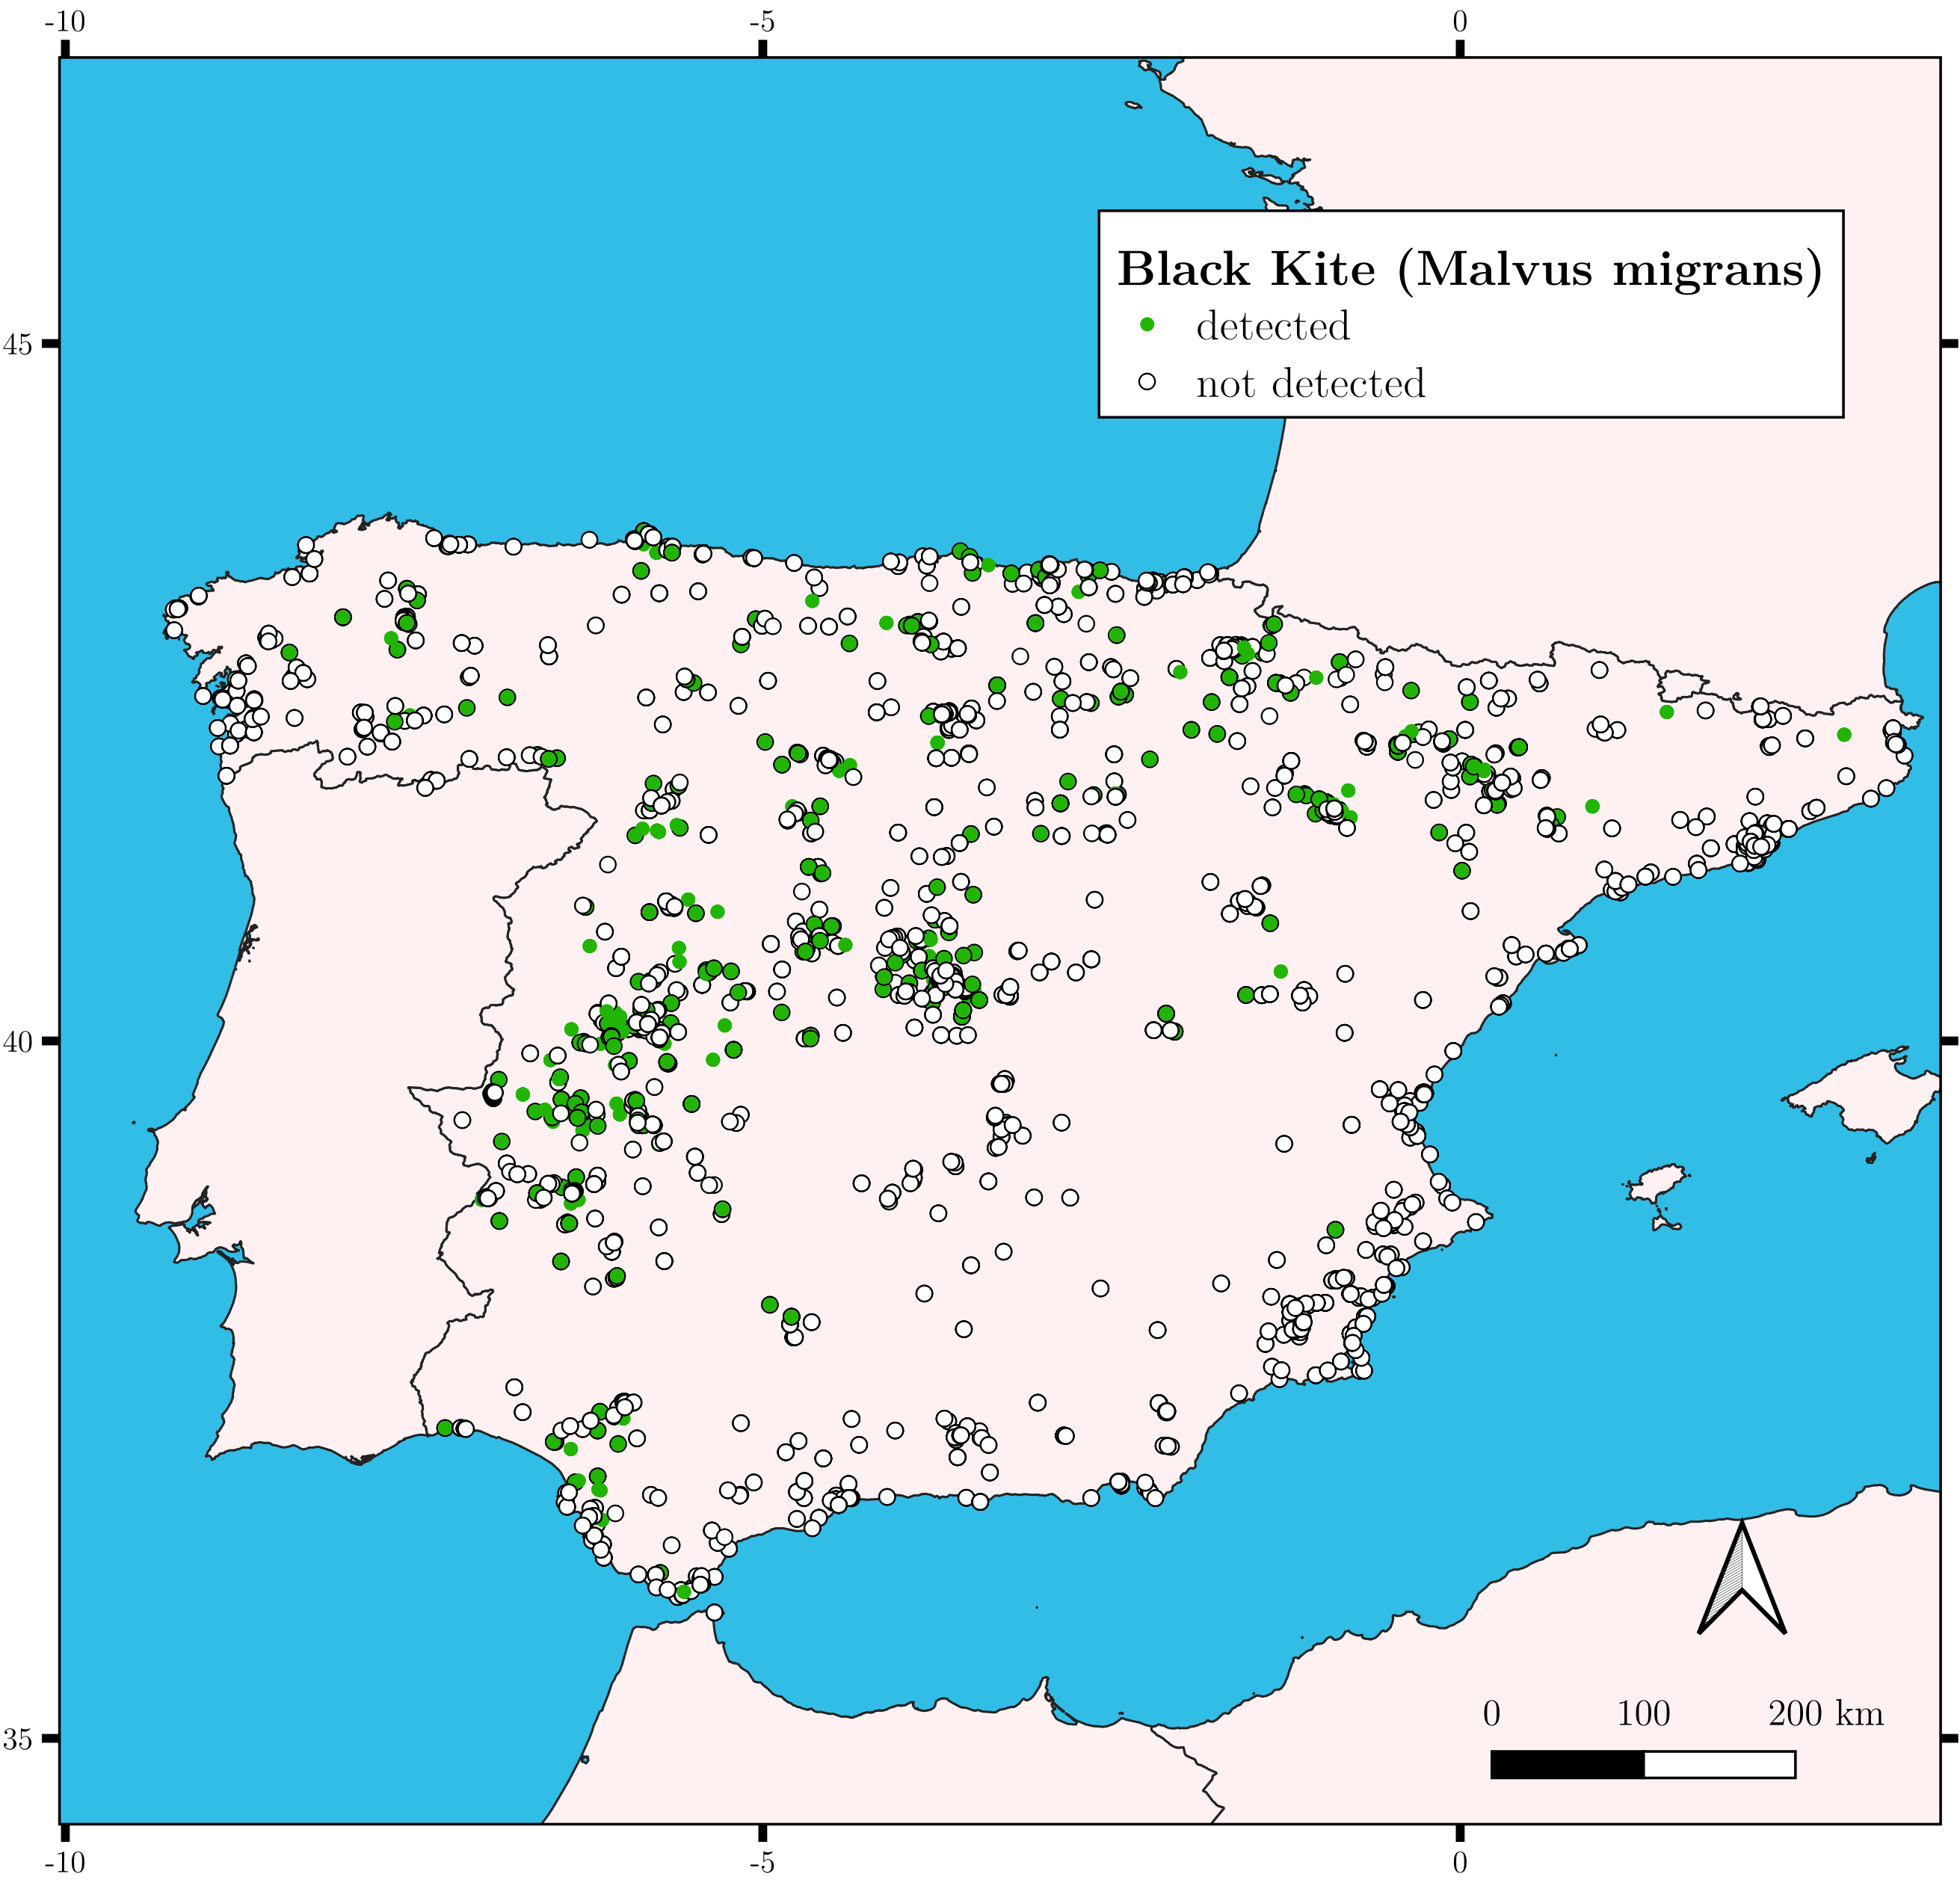
\includegraphics[width=0.6\linewidth]{img/occurences}
	\caption{Detection of the Black Kite in the filtered eBird data set in Spain, each dot represents one observation within the repeated surveys, created with \textcite{QGIS_software}}
	\label{fig:occurences}
\end{figure*}


\subsection*{Selection of best model}
A nullmodel, a model with only detection covariates, a model with only site covariates and a full model (site and detection covariates) were compared with the Akaike information criterion (AIC) and the Akaike information criterion corrected for small sample size (AICc) with \textcite{unmarked}. The model with the lowest AIC and AICc was chosen. 

To compare the stability of the model an average model was build from the best model. Subsets of the best model were chosen with \textcite{Barton2020}, all detection covariates were used as fixed terms (present in all subsetted models). Models were sorted according to the lowest AIC and selected with cumulative Akaike weight \parencite{Wagenmakers2004} larger than 95 \%. The selected models are weighted with the AICs and averaged with \textcite{Barton2020}.

\begin{figure*}[t]
	\centering
	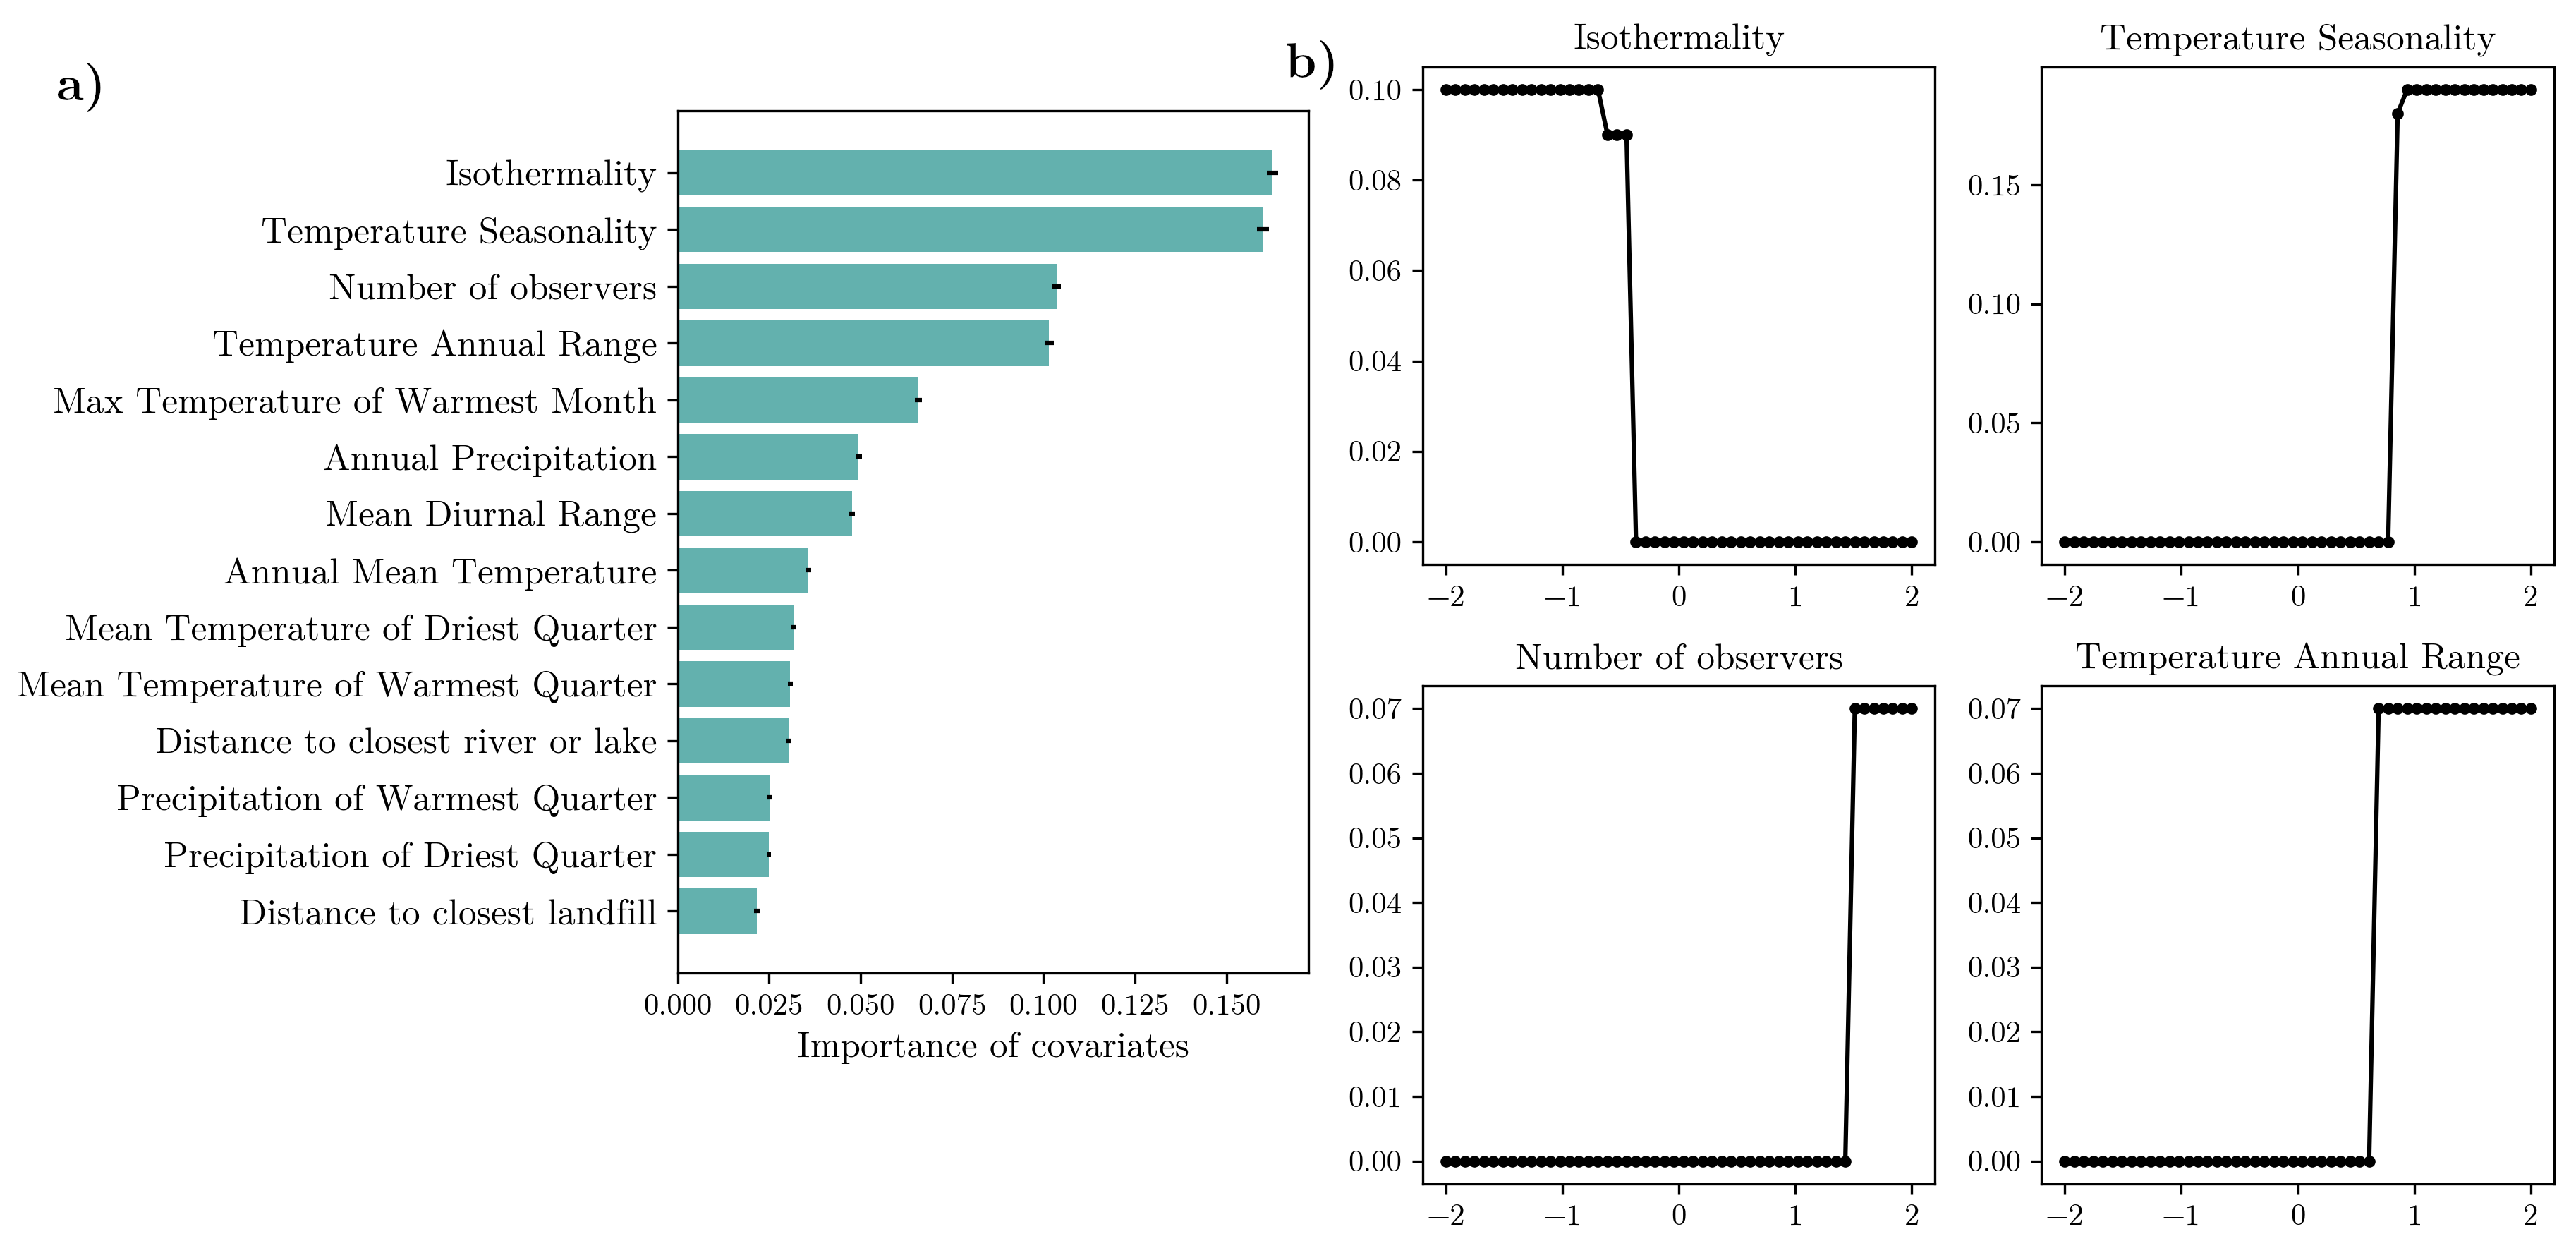
\includegraphics[width=\linewidth]{img/random_forest}
	\caption{Relationship between covariates and detection probability, (a) importance of the covariates in the Random Forests model (only covariates with importance > 0.02 are included), mean importance values of 500 simulation are shown, black lines represent the standard error, and (b) influence of the four most important covariates on the detection probability of the Black Kite in Spain, the y-axis shows the probability, the x-axis the standardized value of the covariate, created with \textcite{matplotlib}}
	\label{fig:random_forest}
\end{figure*}


\subsection*{Model evaluation}
The predictive power of the best model is evaluated with the $R^2$-value \parencite{Nagelkerke1991}. A parametric bootstrapping approach is used to access the goodness of fit \parencite["parboot" function as implemented in][]{unmarked}. From the test results the $\hat{c}$-value was calculated. If this values is noticeably larger than one, it indicates overdispersion of the model. With this $\hat{c}$-value a quasi-Akaike information criterion corrected for small sample size (qAICc) was calculated to see if there are big differences to the calculated AICc. Another goodness of fit as proposed by \textcite{MacKenzie2004} was carried out \parencite[implemented in][]{AICcmodavg}.


\subsection*{Prediction}
Predictions were done with the best model for the mainland of Spain. A map was produced with the predicted occupancy and the standard error of the prediction.
 
Prediction of future climate conditions were done accordingly to existing knowledge about the climate change. The annual temperature will likely rise around 3 °C and the annual rainfall will decrease around 10 \% from 2020 to 2100 \parencite{aemet}. \textcite{ipcc} show under the SSP2 4.5 scenario \parencite{Riahi2017} an increase between 2 and 3 °C and a decrease of total precipitation between 5 \% and 20 \% in different areas of Spain (mean values of 32 models, 2081-2100, relative to 1995-2014). The model agreement is high for the temperature increase, however the signal is not robust for the decrease in total precipitation. These data set is used to model the future occupancy of the Black Kite. The interactive atlas provides regional predictions on a spatial scale of 95 km edge length of a raster cell. GeoTIFFs were downloaded for the change in annual mean temperature and the annual total precipitation (change from 1995-2014 to 2081-2100). These raster files were cropped to the mainland of Spain and resampled to the target resolution (2.5 minutes of a degree). Maps of the changes in the target resolution can be seen in the appendix (see Figure \ref{fig:climate_change}). The change in temperature and precipitation were applied to the respective bioclimatic variables \parencite{Fick2017}. 

We will only incorporate the habitat suitability in relation to climate factors and omit all biological mechanisms that are proposed to play a role for prediction by \textcite{Urban2016} like demography or evolution of a population. It is therefore a simplistic model, but the goal is to catch the main trend.

The effect of the site and detection covariates were tested. Accordingly, all other covariate than the target covariate were set to the mean value and the predictions were done in the range of the target covariate that the model was fitted to. Occupancy probabilities were produced for this range the uncertainty was measured with the standard error.


%\begin{figure*}
%	\centering
%	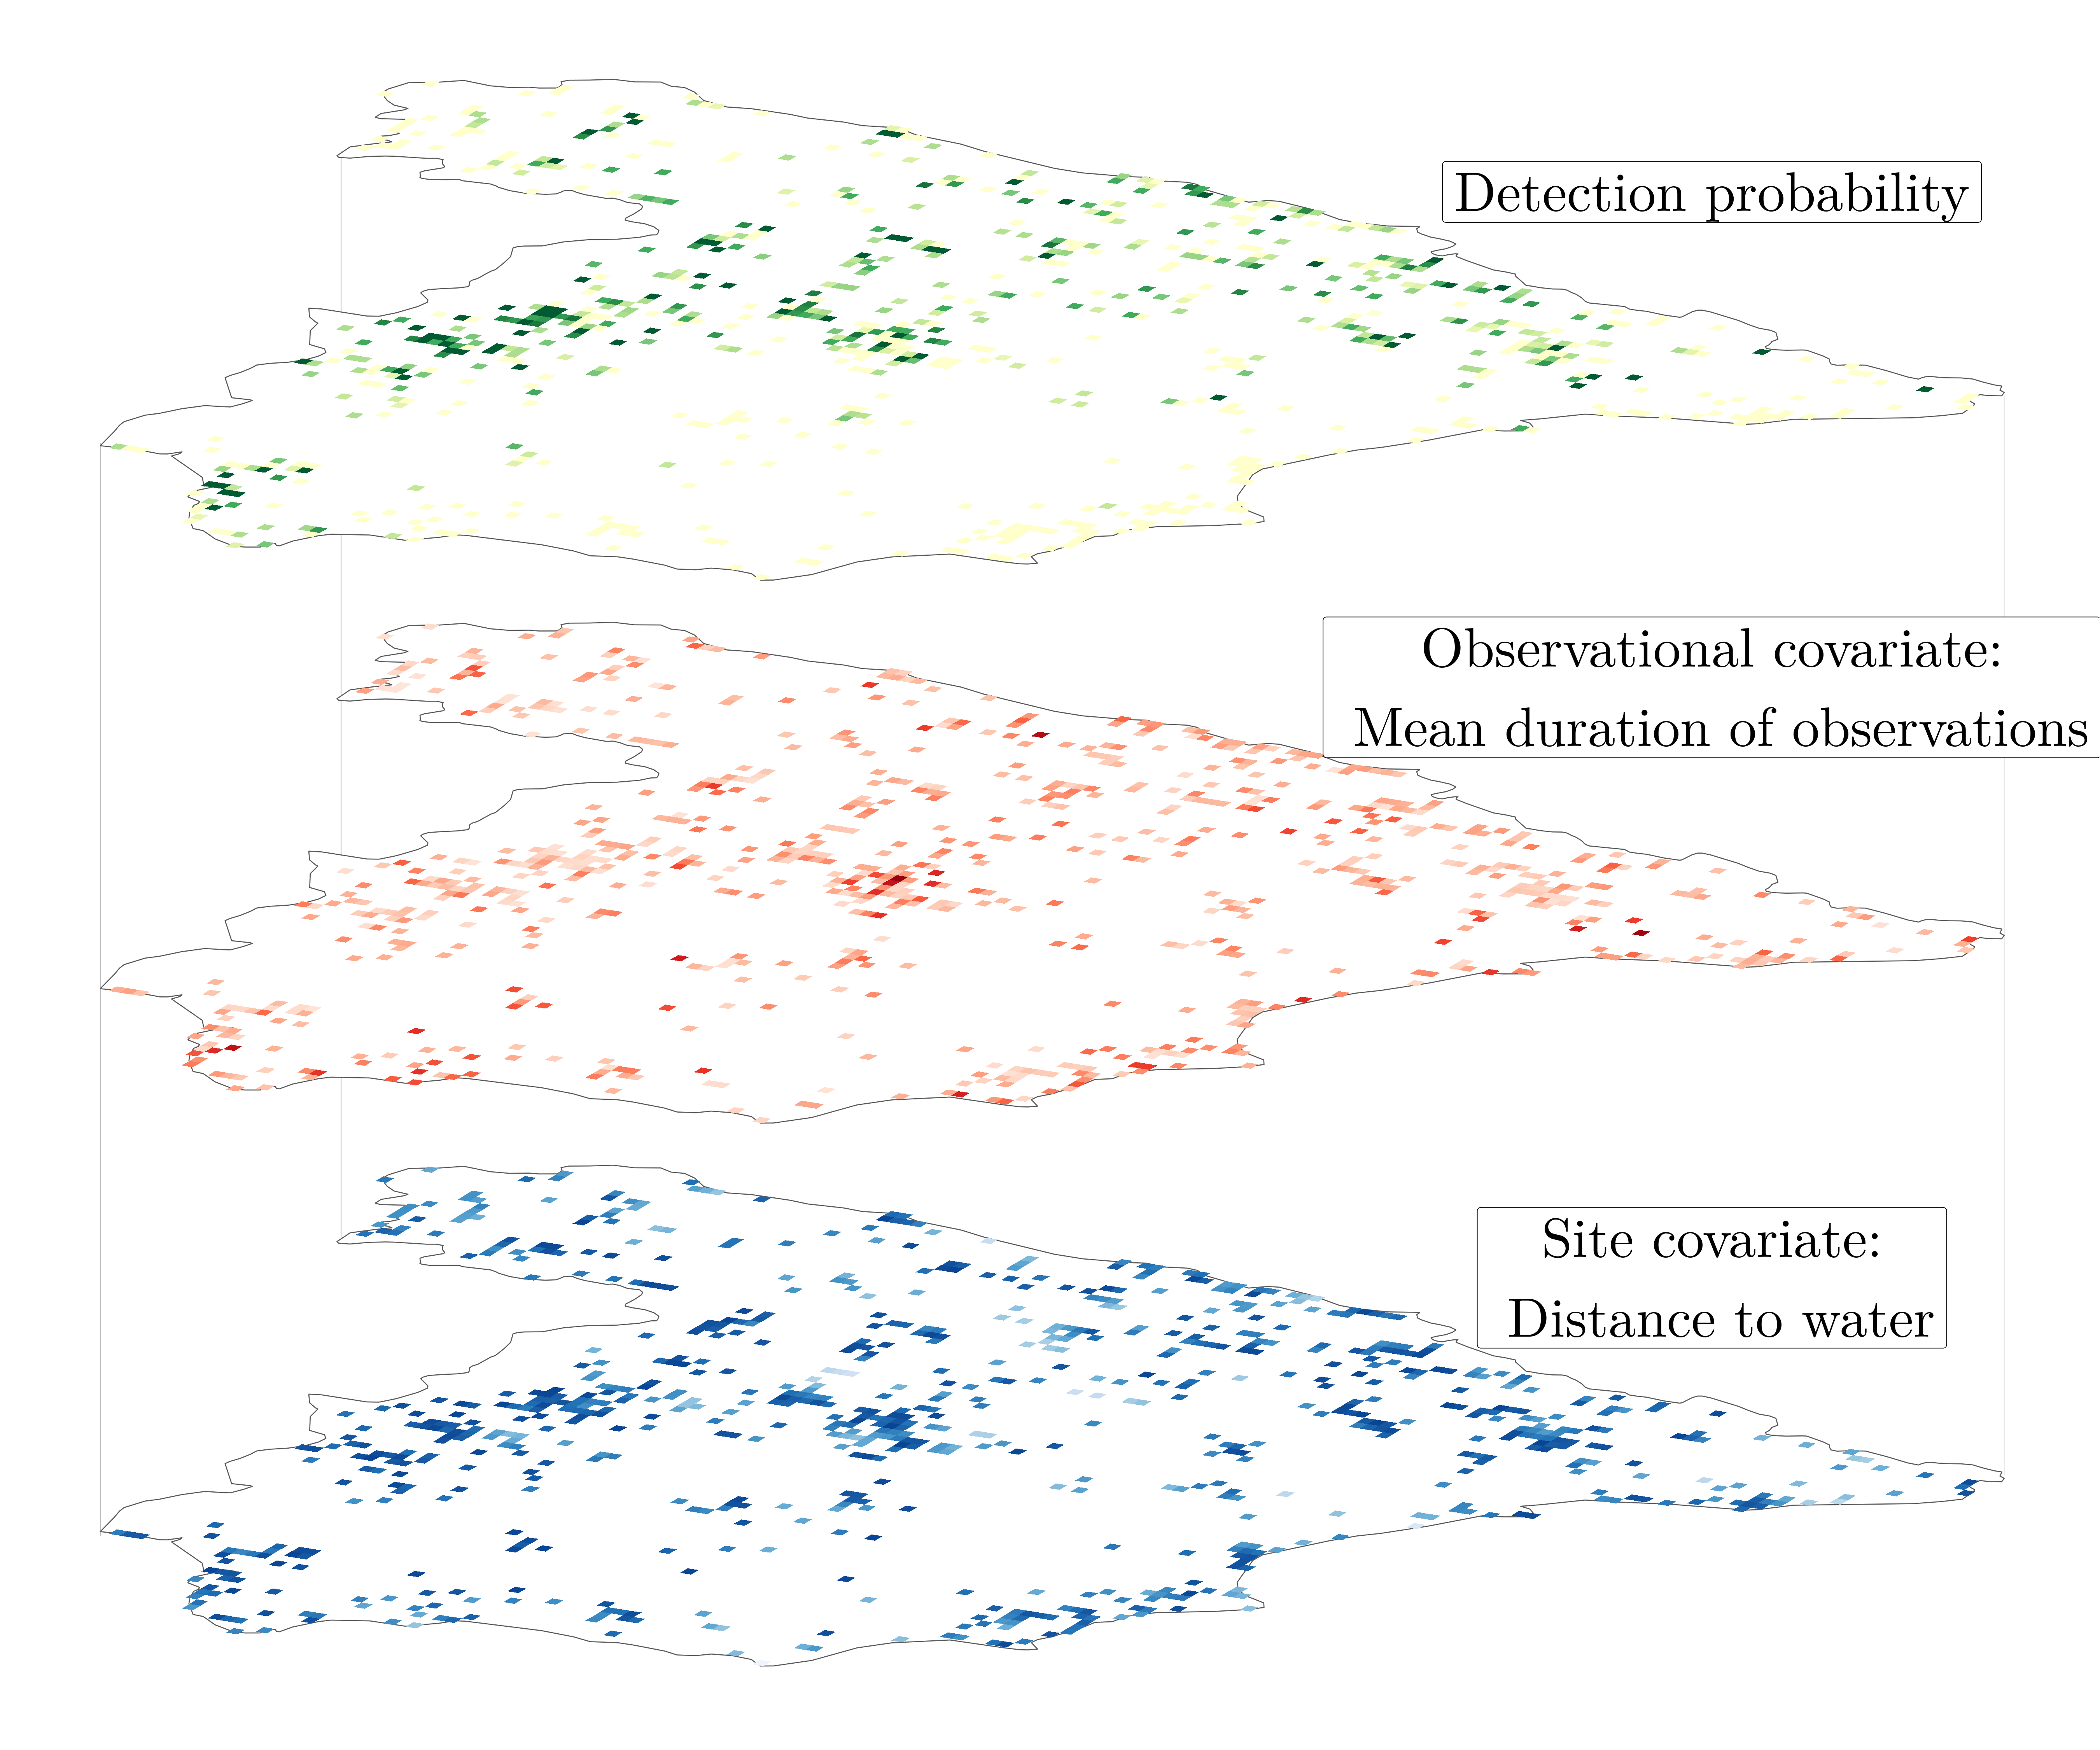
\includegraphics[width=0.7\linewidth]{img/visualization_occupancy_model}
%	\caption[srfs]{Visualization of the model fitting: }
%	\label{fig:visualizationoccupancymodel}
%\end{figure*}

\section{Results}
A map with all filtered observation from the eBird data set is shown in Figure \ref{fig:occurences}. It can be observed that the main distribution is in central Spain. The Black Kite was detected from the coast of the Gulf of Cadiz northwards up to the western Pyrenees. However, in the south-eastern part of Spain detections of the Black Kites are rare.  

\begin{figure*}[t]
	\centering
	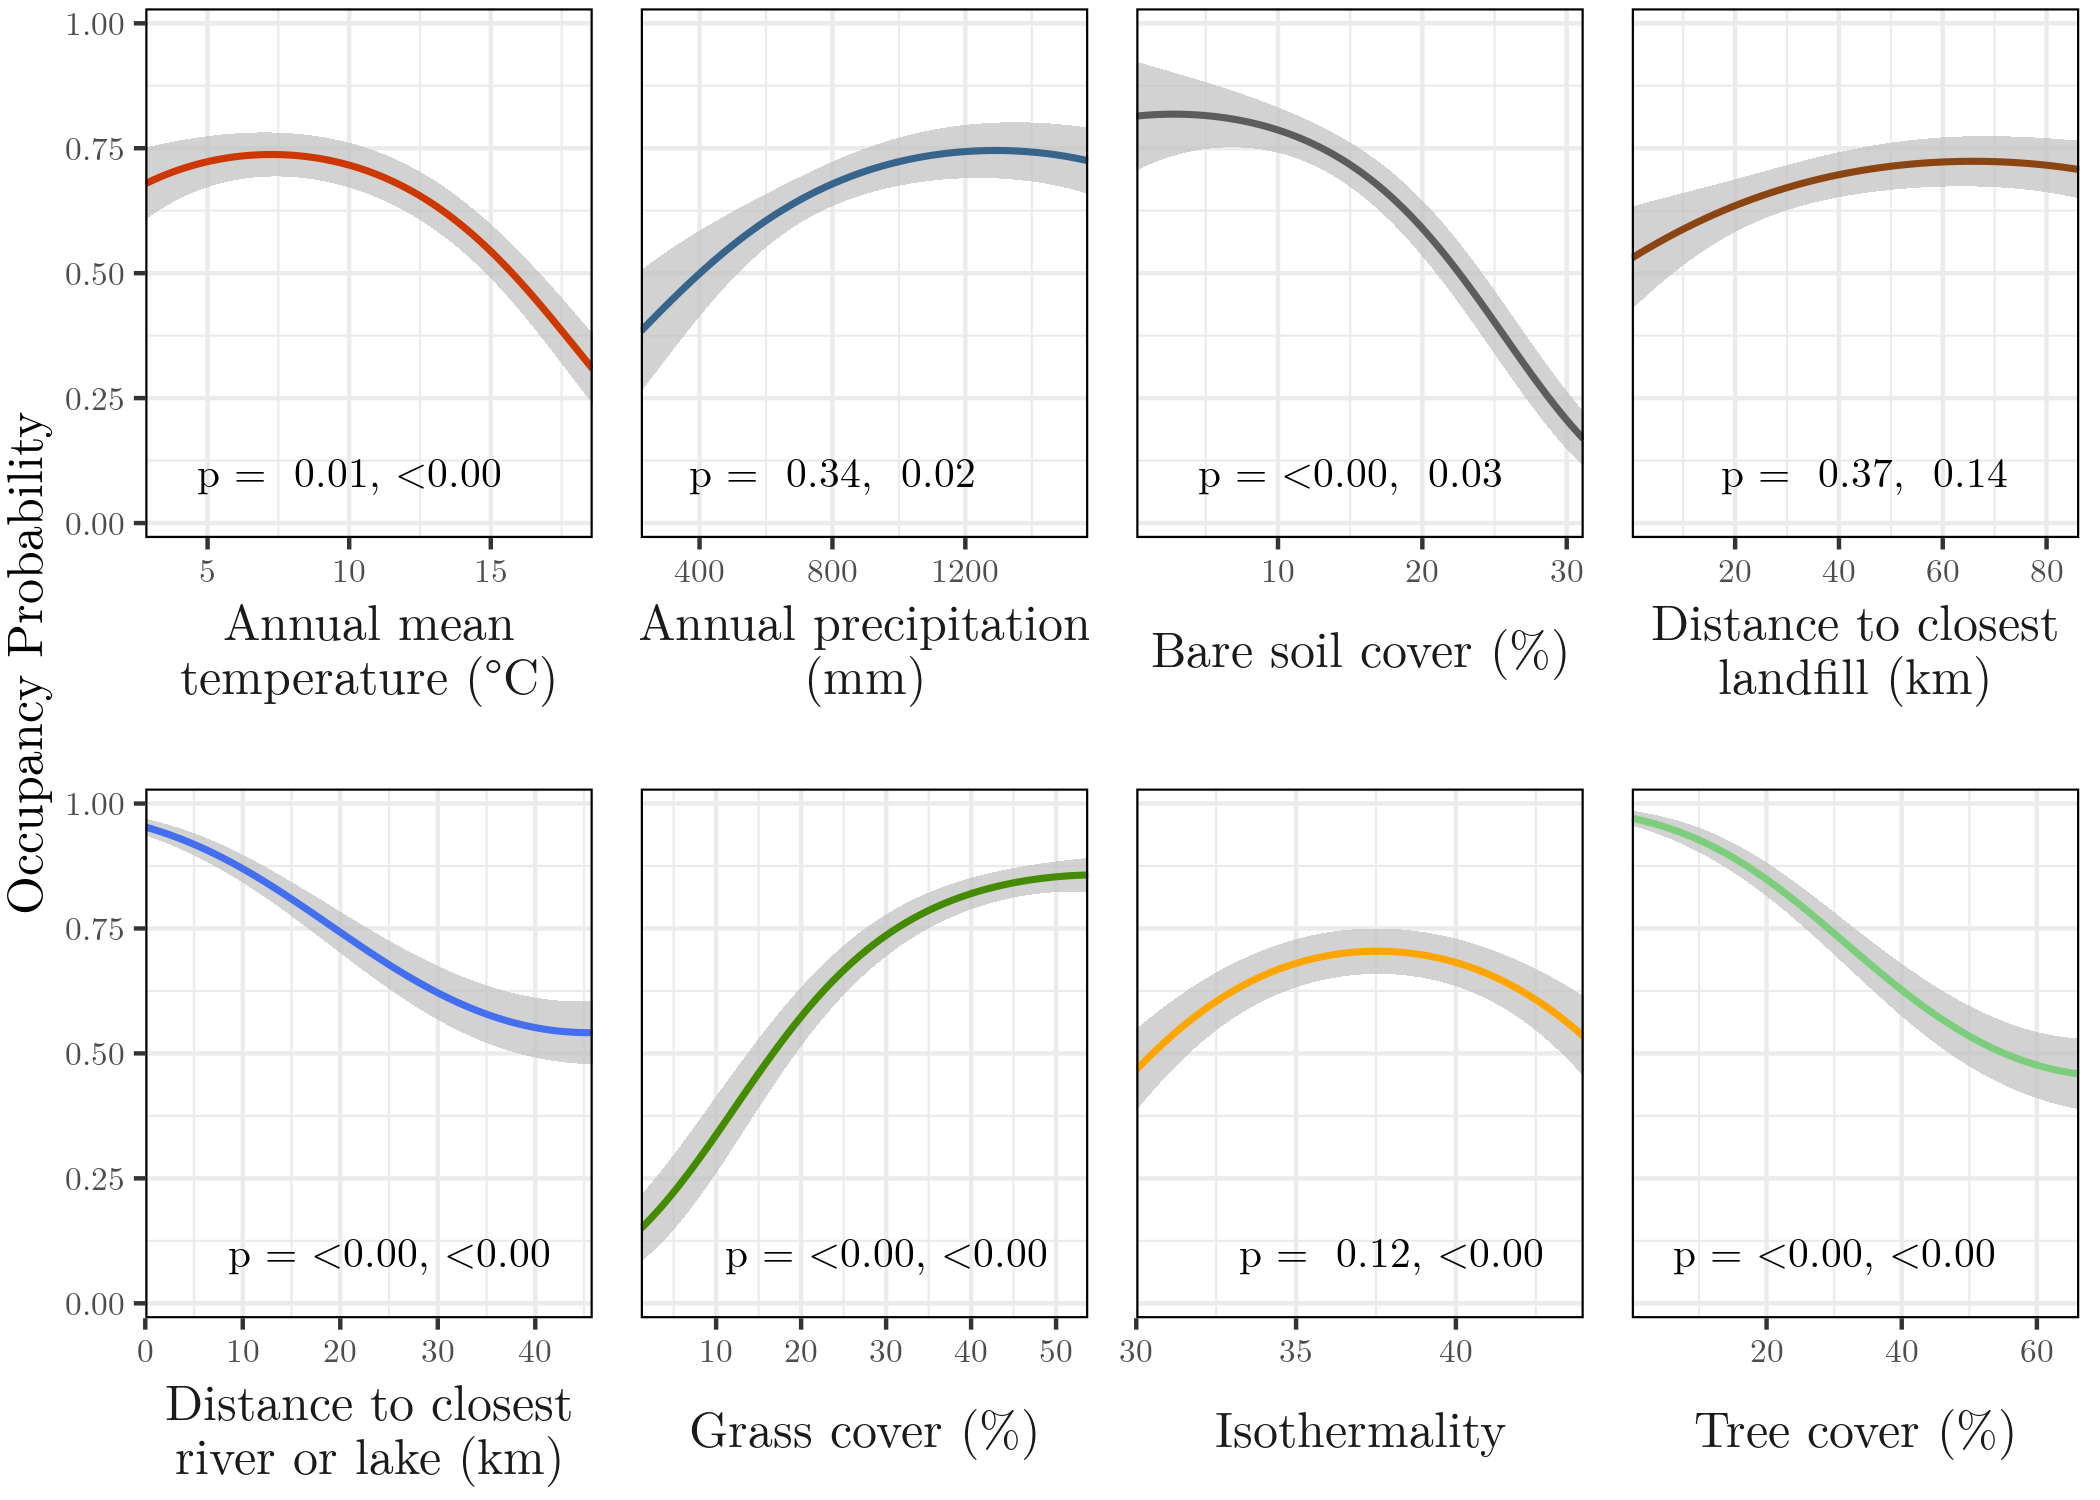
\includegraphics[width=\linewidth]{img/site_covariates}
	\caption{Predicted occupancy of the best model in response to site covariates, for each plot only the focal site covariate was varied, grey areas represent the standard error, the p values show the significance of the first and the second coefficient, created with \textcite{ggplot2}}
	\label{fig:site}
\end{figure*}

\begin{figure*}[t]
	\centering
	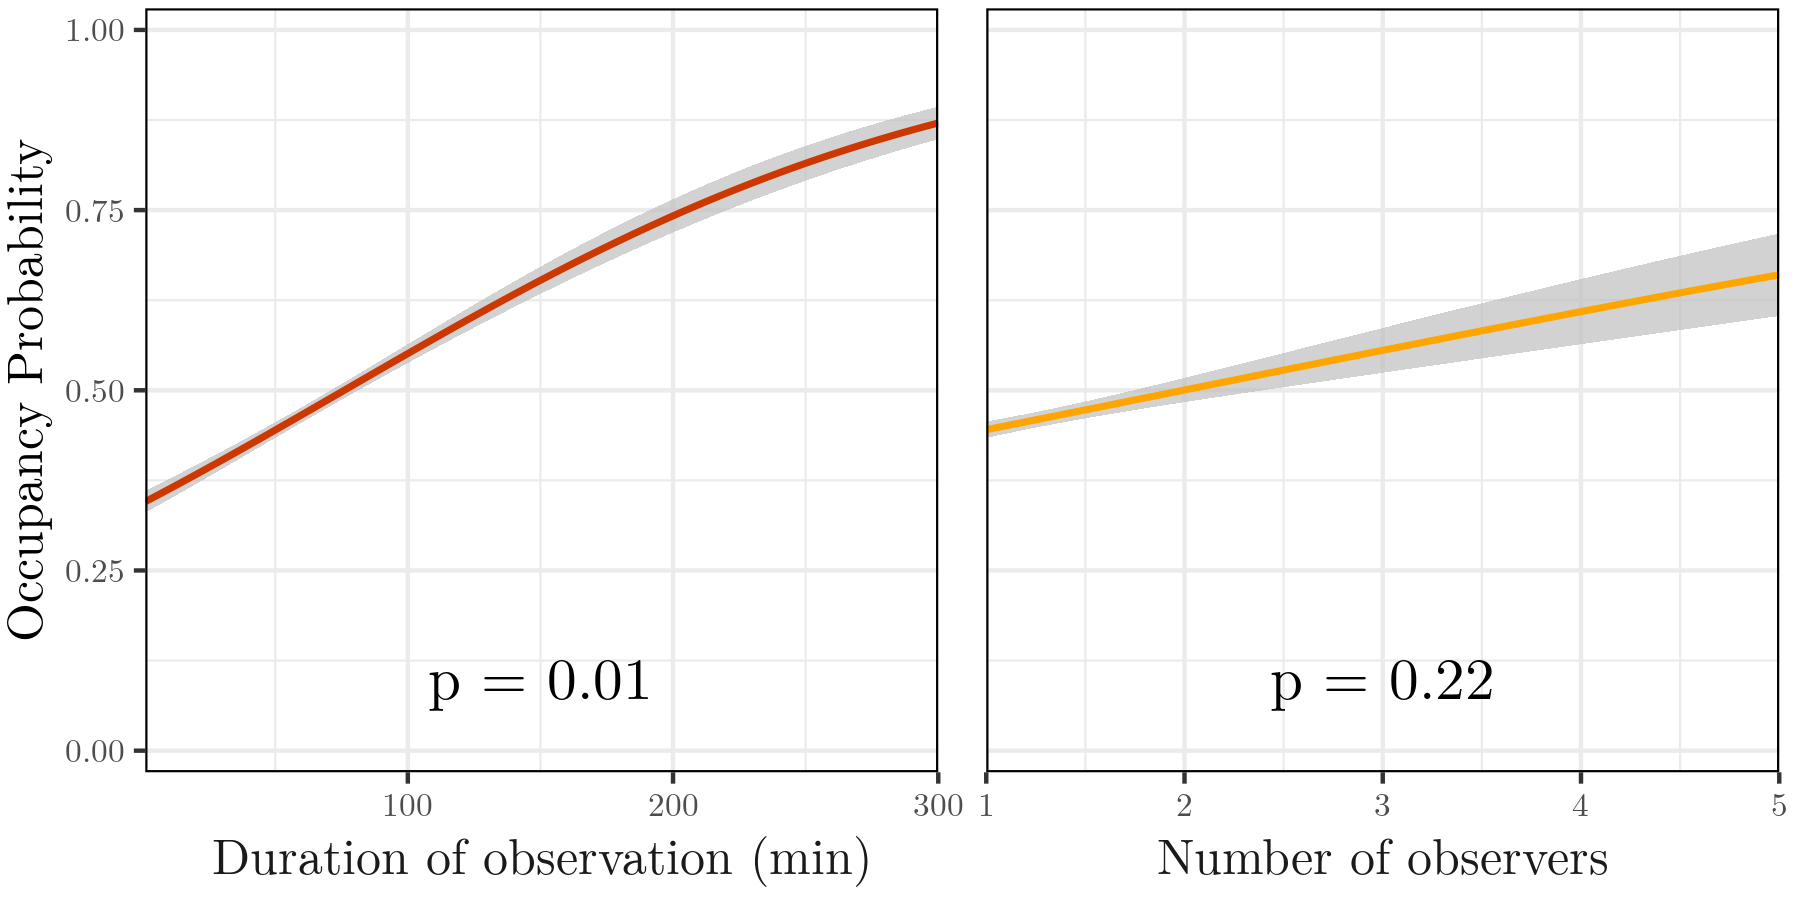
\includegraphics[width=0.8\linewidth]{img/det_covariates}
	\caption{Predicted occupancy in response to detection covariates, for each plot only the focal detection covariate was varied, grey areas represent the standard error, the p values show the significance of the coefficient, created with \textcite{ggplot2}}
	\label{fig:det}
\end{figure*}


\subsubsection*{Exploratory analysis of covariates}
The Random Forests model could explain close to 100 \% of the detection of the Black Kite in the train and the test data set. An overview of the most important covariates can be found in Figure \ref{fig:random_forest}a. 

Especially important are covariates that deal with temperature evenness over the year like isothermality, temperature seasonality and temperature annual range. The only detection covariate that really plays a role is the number of observers. More observers improve the chance to detect a Black Kite (see Figure \ref{fig:random_forest}b). Land cover fractions are not represented under the most important covariates. The annual precipitation is sixth influential covariate. The distance to the closest river or lake and the distance to the closest landfill play minor role.

The four most important factor, namely the isothermality, temperature seasonality, temperature annual range and maximal temperature of warmest month were added as preliminary covariates.   

\begin{figure*}[t]
	\centering
	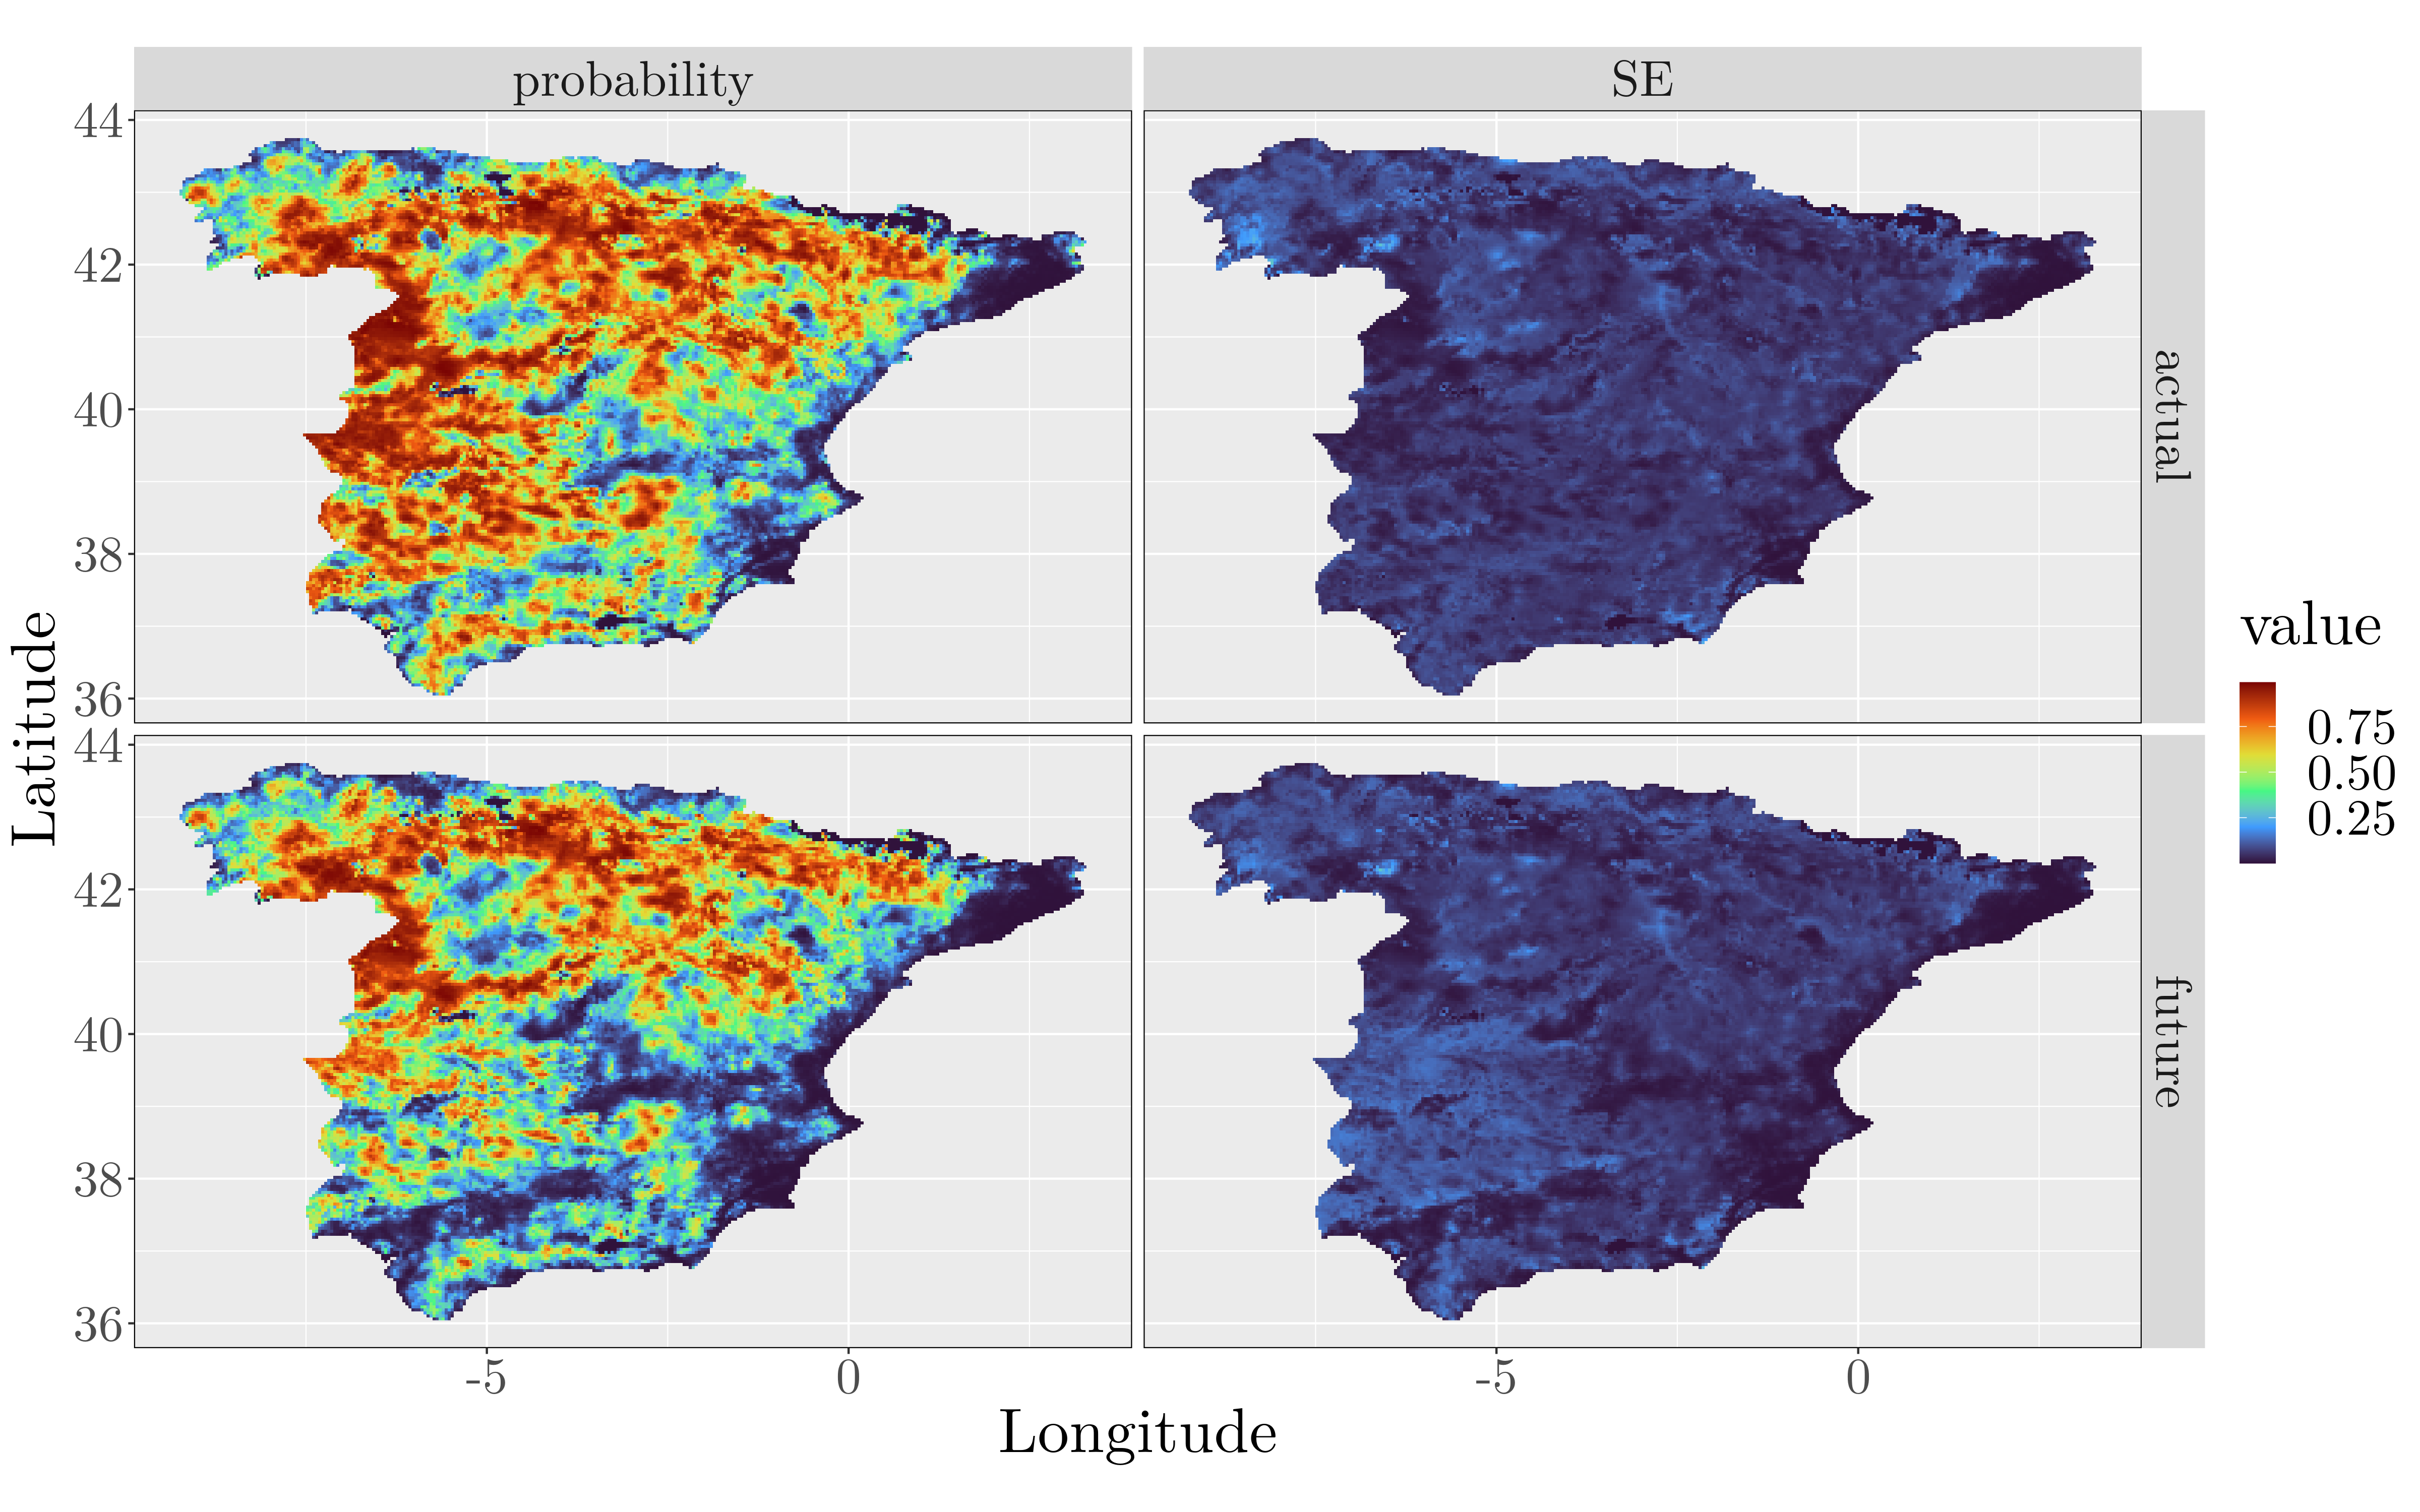
\includegraphics[width=\linewidth]{img/best_model_map}
	\caption{Occupancy map under actual and future climate conditions predicted with the best model, the occupancy probability is shown in the left maps, the corresponding standard error in the plots on the right side, created with \textcite{ggplot2}}	
	\label{fig:map}
\end{figure*}


\subsubsection*{Occupancy model}
Seven site covariates were analysed from the ecological hypotheses and four were added from the Random Forests model. Because of the high collinearity temperature seasonality, temperature annual range and maximal temperature of warmest month were excluded from the final list of covariates. After that the variance inflation factor was for all covariates below 1.9. The highest correlation exists between the tree cover and the annual precipitation (Pearson $\rho = 0.62$). 

The final best model consists of 20 parameters and has an AIC of 4578. The second best model with only the site covariates has an AIC that is 143 higher (delta AIC). The AICc gives roughly the same result. In the best model there are two detection covariates, namely the number of observers and the duration of observation. All site covariates are fitted as polynomials of two degrees. These are the annual mean temperature, the isothermality, the annual precipitation, the bare soil cover, the grass cover, the tree cover, the distance to closest river or lake and the distance to closest landfill. All estimated values of the site covariates are significant different from zero, except the first coefficients of the isothermality and the annual precipitation and both coefficients of the distance to the closest landfill (see Figure \ref{fig:site}). The coefficient of the duration of observation is significant different from zero, however the number of observers not (see Figure \ref{fig:det}).

The occupancy probability shows a positive relation with the grass cover and the annual precipitation. A unimodal relationship can be seen between the isothermality and the annual mean temperature and the occupancy probability of the Black Kite. Bare soil cover, distance to closest lake or river and a high tree cover have a negative influence on the occupancy probability. Both coefficients of the distance to the closest landfill are not significant that is why we cannot see any trend here (see Figure \ref{fig:site}). 

An average model was build from three single models. These are one model with all site covariates except the distance to closest landfill, a model with all site covariates and a third model with all site covariates except the annual precipitation and the closest distance to landfills. These results go inline with the non-significance of the coefficients of the covariates closest distance to landfills and annual precipitation in the full model.

The explained variance in the detection of the Black Kite is 35 \% ($R^2$-value).

The model predicts that 522 out of 1032 grid cells with observations are occupied (51 \%, median best unbiased predictor from occurrence state). In 503 grid cells was the Black Kite detected (49 \%). The \textcite{MacKenzie2004} goodness-of-fit test shows that the model adequately fits the data ($\hat{c} = $ 0.83, $p$ = 1). Also the parametric bootstrap test does not indicate a lack of fit ($\hat{c} = $ 0.97, $p$ = 0.86). The $\hat{c}$-values are below zero, for this reason no QAIC and QAICc are calculated (they have the same values as the AIC and AICc when setting the $\hat{c}$-value to one). 

The mean occupancy probability under actual climate conditions is 52.6 \% (16748 grid cells with occupancy probability $>= 0.5$). The mean occupancy probability decreases and is 37.8 \% under future climate conditions (10290 grid cells with occupancy probability $>= 0.5$). This decrease in occupancy is also visible in the map especially between Sevilla and Madrid (see Figure \ref{fig:map}). In 92 \% of all grid cells there is a lower occupancy probability under future climate conditions, in contrast in only 8 \% of all grid cells the occupancy probability is higher under future climate conditions.

The duration of the observation has a positive influence on the occupancy probability. In contrast, the number of observers does not show a significant result (see Figure \ref{fig:det}).     



\section{Discussion}
Our results imply that the climate change may negatively affect the occupancy of the Black Kite in Spain. 



annual mean temperature, Annual precipitation, bare soil cover, tree cover, grass cover, distance to closest river or lake in line with hypothesis

distance to closest landfill coefficients not significant, even opposite trend 
large landfills have to be covered due to eu law


duration of observation the only significant detection covariate --> maybe other detection covariate more appropriate like the weather at the day of the observation

general reduction of occupancy of the black kite under future climate conditions, very coarse scale of climate prediction, climate is not the only factor that will change, ecology of species may also change.







\end{multicols}